\scanpage{73}
$I'$, $I''$, les $I'_\alpha$ sont des parties de $I$ satisfai-\linebreak sant (7) (des \uline{cribles} de $I$)

Si dans A) on prend $X'=X$, il est plus commode de travailler avec la stratification de $X'$ définie par les $X_i$ avec $i\in I'$ --- il est clair que les conditions (11) relatives à $X'=X_{I'}$ sont satisfaites. Les ``parties cribles'' de $X'$ pour cette stratification, \unsure{ou|—} pour celle induite au sens général des espaces au dessus de $X$, sont les $=^{\mathrm s}$ --- ce sont \inserted{donc} les traces \deleted{\unsure{inverses|induites}} \inserted{sur} $X'=X_{I'}$ des parties-cribles de l'espace stratifié $X$.

Ici, les espaces élémentaires pour la stratification de type $I'$ de \deleted{\unsure{X|\xi}} $X'=X_{\unsure{J'|I'}}$, sont les espaces
\figure{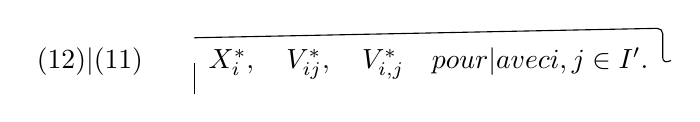
\begin{tikzpicture}
\node[inner sep=5pt] (f) {$X_i^*,\quad V_{ij}^*,\quad V_{i,j}^{\deleted{\unsure{*}}}\quad\text{\unsure{pour|avec} }i,j\in I'.$};
\node[anchor=base east] at ([xshift=-1.5em]f.base west) {$\unsure{(12)|(11)}$};
\draw[rounded corners=2pt] ([yshift=-.4ex]f.north west)--([yshift=.4ex]f.north east)--(f.east)--([xshift=.3em,yshift=.1em]f.east);
\draw (f.west)--(f.south west);
\end{tikzpicture}}

% One cancellation covers this paragraph and the following formula (13).
\deleted{Combinant les deux opérations, on a p.ex. une stratification pour tt ouvert $U'$ d'un $X'=X_{I'}$, avec les espaces \deleted{élémentaires} associés, qui sont donc les}
\[
\deleted{(13)\quad U'\cap X_i^*,\quad U'\cap V_{ij}^*,\quad U'\cap V_{ij}\qquad(i,j\in I')}
\]

\margin{72}
